\documentclass[10pt, a4paper]{article}
\usepackage{fullpage}
\usepackage{graphicx}
\usepackage{subcaption}
\usepackage{wrapfig}

\DeclareGraphicsExtensions{.jpg, .png, .pdf} %.jpg .png .pdf

\setlength{\parskip}{0.2cm}
\setlength{\parindent}{0cm}

\begin{document}
\title{Project Evaluation
\\ 3D Heap Visualisation}
\author{Aviv Beeri, Briony Goldsack, Ying Jiang, 
\\ Oliver Myerscough, Anna Thomas, Eleanor Vincent}
\maketitle


\section{Introduction}

An object-oriented software application creates complex structures on the heap during its lifetime. Debugging object-oriented software often involves thinking about how the heap evolves as a program runs. The aim of our group project is to design a tool which supports visualisation of the heap of a running Java program as a 3D scene which can be navigated by the software developer by moving around as if in a first person shooter game.

This report aims to describe how we have quantitatively evaluated the work we have produced and the techniques we have employed to measure and analyse our results. We will discuss the particular qualities of our project that are most important in carrying out our evaluation, the metrics we have used, and the data we have gathered. 

\section{Project Evaluation}

There are several qualities within our project that are particularly important when carrying out evaluation on the Heap Visualisation tool and assessing its success as a product. Firstly, we feel that the performance, intuitiveness and functionality of the debugger aspect is very important to our project as this is the foundation of our tool and should behave smoothly and reliably. We feel that another important feature of our project is the graphical visualisation of the heap itself. It was imperative that the visualisation had the qualities such as being informative to the user, intuitive to use and visually appealing so that we can satisfy our stakeholders as identified through the requirements and customer processes. 

We have employed a few different methods to evaluate what we have produced and the assess the important qualities we view as necessary to the project. Primarily, we wanted to assess the usability of our product as this was a key feature of both the debugger GUI and the interactive visualisation of the heap. There were several options open to us as to how to do this: hall-way testing, discussion groups. In order to quantify our results, we decided the best approach was to use a questionnaire. As one of our team members is a UTA we thought that this would be the perfect audience with which to test whether our tool is intuitive enough for inexperienced users. Unfortunately it is still too early for us to test with first years, as they have only just started programming in Java with objects are not ready to gain from using our tool. We plan to perform initial usability testing with them in the coming week.

\section{Testing}
Our automated build process and test suite has enabled us to continuously and quantitatively assess the quality and correctness of our code as we have progressed with the project. The Travis Tests indicate the number of failing builds.

\section{Data Collection}
To further improve on the user experience of our tool, we could use analytic tools to record some quantitative data on how users interact with the product. These would include the amounts of idle time between mouse clicks, recording the path of a user through the program, where they get stuck and perhaps even using some A/B testing to try different program layouts\textsuperscript{\cite{opt}}. This data would allow us to see areas that would need improvements, but the disadvantage is having to actually implement the mechanisms for collecting these analytics, so it is unlikely that we will use this particular technique to gather feedback from potential users. However, after the project is completed, we could use it for further improvements. 

\subsection{Questionnaire}

If the project is to be a success, it is vital that all customers we have targeted find the system intuitive and useful. This is challenging as they come from a wide range of backgrounds; the lecturer with considerable knowledge of programming; the first year student with some knowledge of the same; the gamer, who may well have little knowledge of, or interest in, programming. We have written a questionnaire for our testers to fill out. This allows us to collect structured data which will be much easier to analyse than organic interview notes. The questionnaire first establishes who the user is and their current level of knowledge. We then ask if they could use the program to do the tasks it is designed for; evaluating our project’s functionality. Finally, we ask if they could interpret the results of the 3D heap visualisation.

\begin{wrapfigure}{r}{0.5\textwidth}
        \centering
        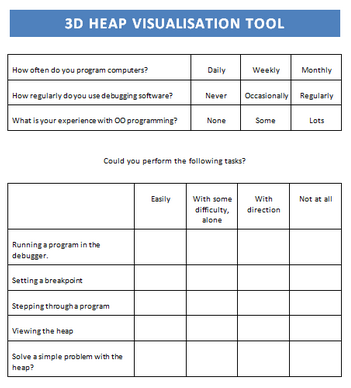
\includegraphics[scale=0.5]{images/evaluation/q.png}
        \caption{Team Questionnaire}
\end{wrapfigure}

By channelling responses to each question into categories we make our analysis of results straightforward. We can easily differentiate between an unclear interface and lack of understanding in the user by separating results based on the first section of questions. If someone who has never used a debugger has trouble setting a breakpoint that is to be expected. If an experienced programmer cannot figure it out we have a usability problem. The results of our questionnaire could be represented as a series of bar charts to aggregate the collection of data and a form easy to analyse. 

The disadvantage of this approach is rigidity in response format. We can encourage testers to write down any opinions they have that the questions we pose have not allowed them to express. When reviewing each feedback sheet we take note of these comments. 
We plan to perform multiple rounds of user evaluation using this questionnaire. This will tell us whether the changes we have made have been effective in improving the system. By cross referencing improvements in results with actions taken over that period we can identify the changes that have been most beneficial to users. Ali wants to use the tool in his lectures. After the course, we could ask students who used it to answer the questionnaire, providing further data and allowing for more improvements. We can even have discussions with students while they are learning to use the product to learn more about their experiences.

\section{Data Visualisation}

Throughout the development process, we have sometimes found it necessary to visualise data to help others to understand it. One example of this is with our testing process. Our automated build process and test suite has enabled us to continuously and quantitatively assess the quality and correctness of our code as we have progressed with the project. The Travis Tests quickly indicate the number of failing builds, while the test results can be viewed in an XHTML format as a visual aid to other team members of issues within the code. A further prominent example of visualising data used within our project to make it easier to interact with and understand is our debugger GUI. We had initially not planned for there to be an interface other than a simple console application to interact with the program’s heap we are visualising, however, following supervisor discussions, it was soon realised that a GUI would allow everyone (team members, supervisor and eventual customers) to better understand the product and how to use if effectively. We have evaluated our team performance and development process in a number of visual ways to gain useful insights into our progress and communicate with stakeholders such as our supervisor, for example, the burndown chart. 

\section{Team Performance}

To evaluate how our development team has functioned during the project we have performed 360-degree feedback, feedback that comes from members of an individual’s immediate work circle. As we used Trello for project management we can use it’s Kanban flow to analyse our response time to adding new features and ideas, this will allow us to know roughly how long it is taking us to produce a new feature once it’s been asked for.

We tried to maintain high performance in our team\textsuperscript{\cite{semantia}} by holding weekly team meetings, providing feedback in real time and negotiating the short-term and long-term goals of our project together. In our meetings we have regularly discussed the use of agile development as at the beginning of our project we agreed to complete weekly sprints to implement new features, however in practice we found that due to the varied work load of our other subjects this was an unreasonable ask. 

\begin{wrapfigure}{r}{0.5\textwidth}
        \centering
        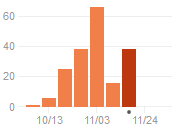
\includegraphics{images/evaluation/commit_freq.png}
        \caption{Commit Frequency}
\end{wrapfigure}

For example, some weeks all team members would have multiple other pieces of coursework to complete, and other weeks many would have a much lighter work load. This meant that some weeks we managed to implement all the features we intended to and during other weeks the project was stalled while members finished other pieces of work, you can see this behaviour from our git commits graph.


To compensate for this we decided not continue using set sprint times but to carry on meeting regularly to report back on progress in each area of the project and to allow team members to raise any issues they had, for example, some members were unsure how the debugger was used and this issue was discussed and resolved in a project meeting.

We have elected not to analyse group performance by the number of lines of code written as this is not a useful metric on it’s own. In practice, Code Style Checking proved to be unhelpful because it was introduced mid way through the project, resulting in a large number of unimportant warnings being raised about our reasonably consistent code style. It was also easy to integrate into our build process, but was not helpful because everyone just ignored the checkstyle warnings. If we had prevented the checkstyle from halting the build it would have stalled the project by a number of days, wasting valuable time.

\subsection{Burndown Chart}

A burndown chart is a graphical representation of work left to do versus time, we split all our major features up into their component tasks and plotted them.

\begin{figure}[h]
        \centering
        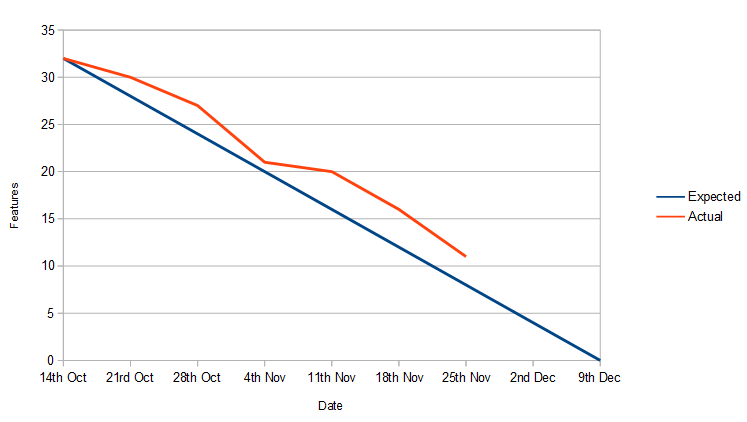
\includegraphics[scale=0.5]{images/evaluation/burndown.png}
\end{figure}

As you can see from the graph we are close to being on track to the expected line, however we know from the previous GitHub commit graph that all our team members were busy somewhere between the 3rd November and 24th November, this matches with our data from our burndown graph as much less work was done around then. One important use of our burndown chart as a tracking tool of our progress throughout the project has been to communicate with our internal customer and supervisor. Furthermore, we have been able to mitigate the risk of schedule overrun, an  important metric in product management\textsuperscript{\cite{burndown}}. We saw few downsides with the upkeep of a burndown chart as it was relatively simple to maintain and enabled us to see if we are falling behind too far. 

\subsection{Kanban Flow (Trello)}

\begin{wrapfigure}{r}{0.5\textwidth}
        \centering
        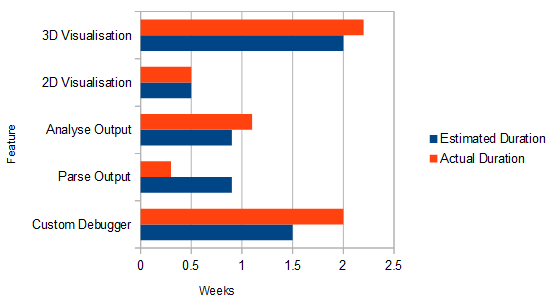
\includegraphics[scale=0.5]{images/evaluation/duration.png}
        \caption{Project Duration}
\end{wrapfigure}

Initially we used  planning poker to estimate how long each major feature would take to implement. Now using data from Trello we can map our estimates to the time between putting a ‘todo’ note up and completing it on Trello, this is shown in the bar chart shown right\textsuperscript{\cite{kan}}.

As we can see from the chart we generally underestimated how long it would take us to implement a basic version of each feature in the project, this data has been useful as it made us acknowledge that our estimates may not always be accurate and we need to allow for slightly more time to complete any new features.

\subsection{360-degree feedback}

360-degree feedback\textsuperscript{\cite{jj}} is feedback that comes from members of an employee's immediate work circle, it includes direct feedback from our peers and supervisor, as well as self evaluation. Sometimes feedback from external sources such as customers is included but this would not be useful for our evaluation as we have not been working closely with an external client. We believe 360-degree feedback is more beneficial in our situation than traditional performance appraisal (where we would only be reviewed by our supervisor) based on the idea that anonymous feedback from multiple sources is more well-rounded than direct feedback from a single source. A downside of 360-degree feedback is what to do in the case of conflicts- when there differing opinions- and who should solve them. This is particularly poignant as our feedback was all anonymous. Furthermore, there is no certainty that our feedback is reliable and truthful, which limits the usefulness of the data collected\textsuperscript{\cite{360}}.

\begin{figure}[h]
        \centering
        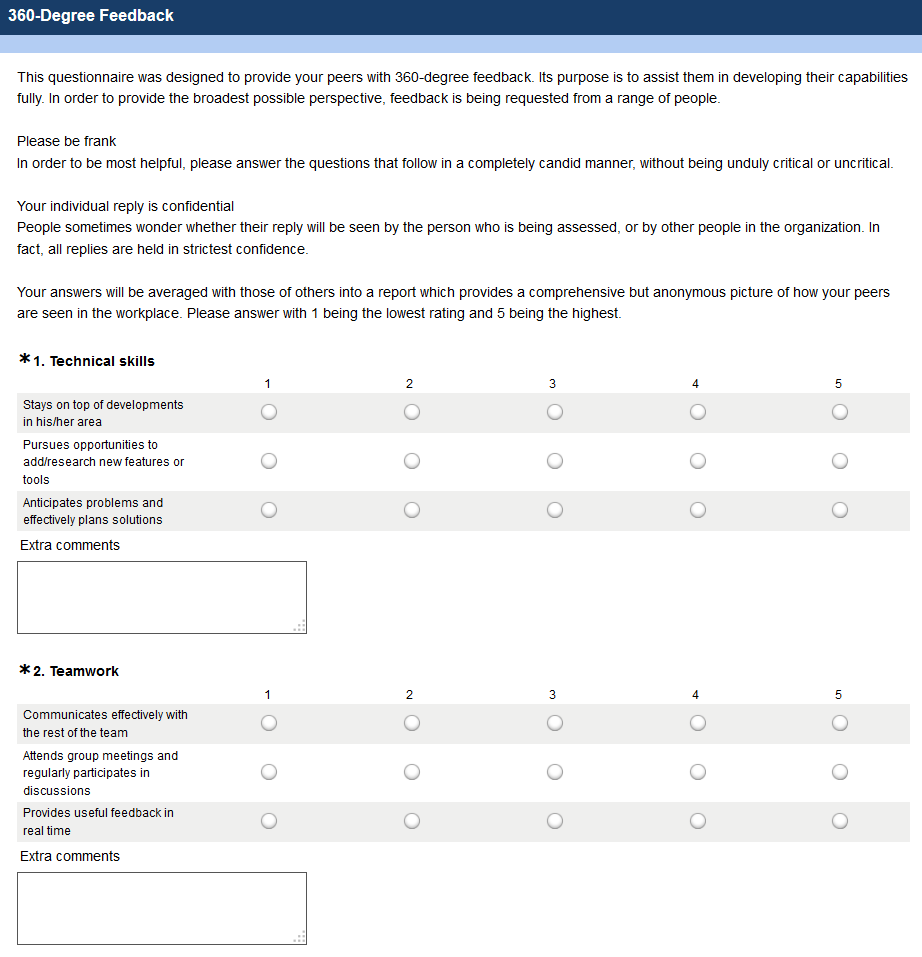
\includegraphics[scale=0.5]{images/evaluation/360_feedback.png}
\end{figure}

\begin{wrapfigure}{r}{0.5\textwidth}
        \centering
        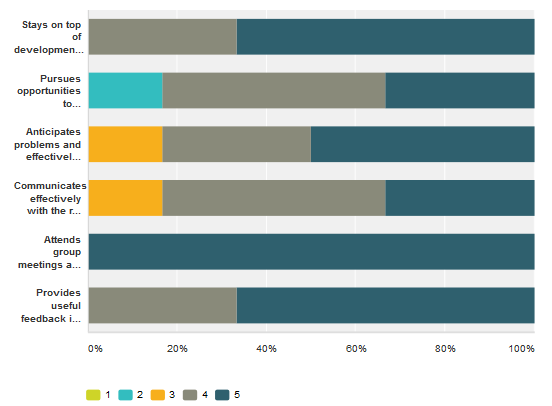
\includegraphics[scale=0.5]{images/evaluation/survey.png}
        \caption{Survey Results}
\end{wrapfigure}

We used SurveyMonkey to ask our team to give feedback on how they believed the rest of the team to be performing. We asked about technical skills such as how they were performing in relation to the features they were implementing and how well they were working as part of a team. The results graph shown is just for one person’s feedback, with 1 being the lowest and 5 being the highest score they could have received in relation to that area. 

This survey highlighted the fact that while as a group we are on track for development, we could improve our communication in the group to avoid some members not understanding parts of the project or having to explain things twice when members aren’t in meetings. The feedback we gained from performing the evaluation will be used to plan the future development of our product as we are able to see where each person’s strengths lie in the project.

\begin{thebibliography}{9}

\bibitem{alicja}
  Alicja Nieborak, 
  \emph{Project planning: Evaluation plan},
  \\ http://www.jisc.ac.uk/fundingopportunities/projectmanagement/planning/evaluation.aspx
 
\bibitem{semantia} 
  Semantia, 
  \emph{How to Evaluate and Appraise Team Performance},
  \\ http://www.semantia.com.au/articles/productivity/how-to-evaluate-and-appraise-team-performance-in-virtual-teams/

\bibitem{jj} 
  Jack Zenger and Joseph Folkman, 
  \emph{Getting 360 Degree Reviews Right}, 
  \\ http://blogs.hbr.org/2012/09/getting-360-degree-reviews-right/

\bibitem{opt}  
  \emph{Optimizely’s explanation of AB-Testing},
  \\ https://www.optimizely.com/ab-testing

\bibitem{kan} 
  \emph{What is Kanban?},
  \\ http://www.everydaykanban.com/what-is-kanban/
  
\bibitem{burndown} 
  Nitin Mittal, 
  \emph{The Burndown Chart}, 
  \\ http://www.scrumalliance.org/community/articles/2013/august/burn-down-chart-{\%}E2{\%}80{\%}93-an-effective-planning-and-tracki
  
\bibitem{360} 
  Mary Vinson, 
  \emph{Pros and Cons of 360 degree feedback}, 
  \\ http://www.star360feedback.com/the-pros-and-cons-of-360-degree-feedback-making-it-work

\end{thebibliography}

\end{document}
